\begin{frame}{Setup}
  `Realistic scenario': Take data from a 2D convection-diffusion system
  \begin{align*}
    \diffp{c}{t} + u \grad{c} &= \nu \nabla{c}, \quad t > 0,
    \quad (x, y) \in \Omega^\circ
  \end{align*}
  where $\Omega = [0, L_x] \times [0, L_y]$ and $u$ solves
  \begin{align*}
    u &= -k \grad{p}, \\
    \grad \cdot u &= 0, \\
    k &\sim \log \mathcal{N}(0, s(x_1, x_2)),
  \end{align*}
  where $s$ is a squared-exponential covariance function.  Observations are
  \begin{equation*}
    d_{jk} = \bar{c}(x_j, t_k) + \eta_{jk},
    \quad \eta_{jk} \sim \mathcal{N}(0, \sigma_{jk}^2)
  \end{equation*}
  where
  \begin{equation*}
    \bar{c}(x, t) = \frac{1}{L_y} \int_{0}^{L_y} c(x, y, t) \ud y.
  \end{equation*}
  We want to model the average (upscaled) behaviour of $\bar{c}$.
\end{frame}

\begin{frame}{Setup}
  Upscaling the convection-diffusion equation (reality) we get:
  \begin{equation*}
    \diffp{\bar{c}}{t} + u_1 \diffp{\bar{c}}{x} + \diffp{}{x}\left(\overline{u_1' c'}\right) = \nu \diffp[2]{\bar{c}}{x}
  \end{equation*}
  Same initial and boundary conditions as reality.
  \begin{itemize}
    \item Just like RANS, upscaling yields a new system with an unclosed term
    \item We need a model for this term.  Know gradient diffusion inadequate, so
      try fractional operator (similar to above formulation):
      \begin{equation*}
        \diffp{ }{x}\left(\overline{u_1' c'}\right) = -\gamma \diffp[2]{\bar{c}}{x} + \beta \mathcal{L}^{\alpha} \bar{c}
      \end{equation*}
      where $\mathcal{L} = -\diffp[2]{ }{x}$.
  \end{itemize}
\end{frame}

\begin{frame}{Likelihood function for fractional operator}
  \begin{figure}
    \centering
    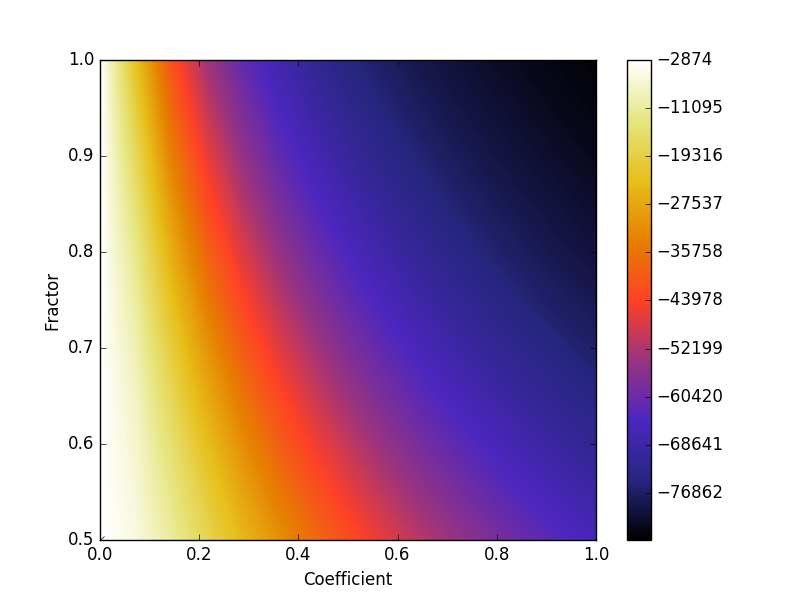
\includegraphics[width=0.7\textwidth]{figs/gridded3D_lp03_sig30_nup05.png}
  \end{figure}
  Very insensitive to fractor $\alpha$ and we basically get back pure diffusion.
\end{frame}

\begin{frame}{Results for general shift-invariant linear operator $\mathcal{L}$}
  \begin{figure}[h]
    \centering
    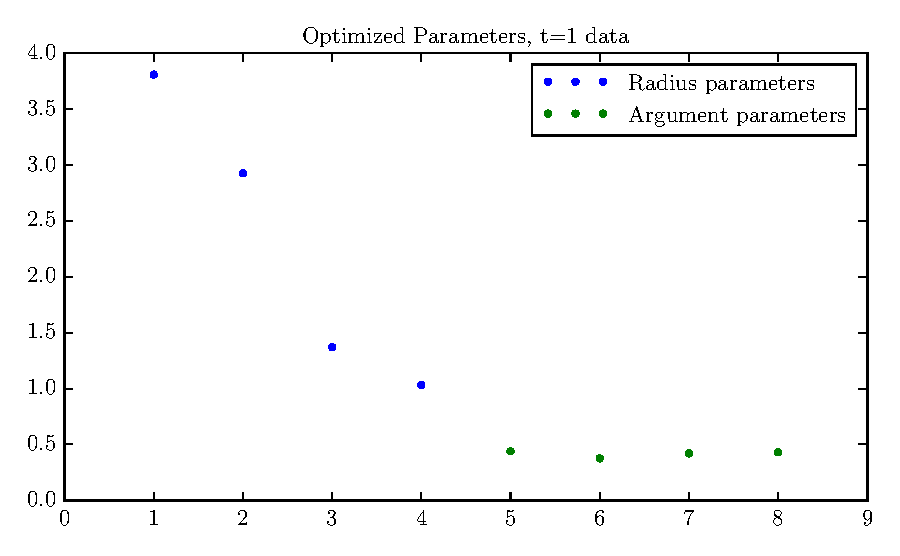
\includegraphics[scale=0.8]{figs/params_t1.pdf}
  \end{figure}
\end{frame}

\begin{frame}{Predictions with general $\mathcal{L}$}
  \begin{figure}[h]
    \centering
    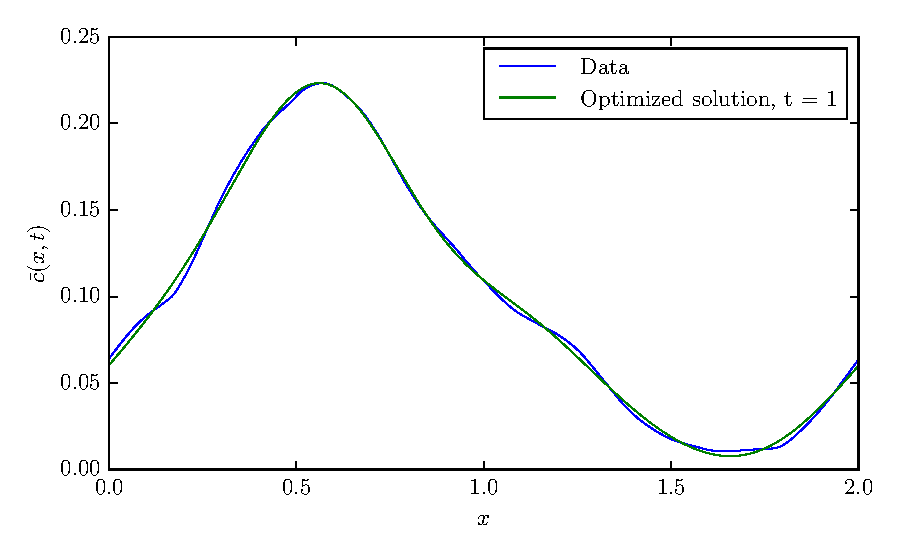
\includegraphics[width=0.4\textwidth]{figs/solns.pdf}
    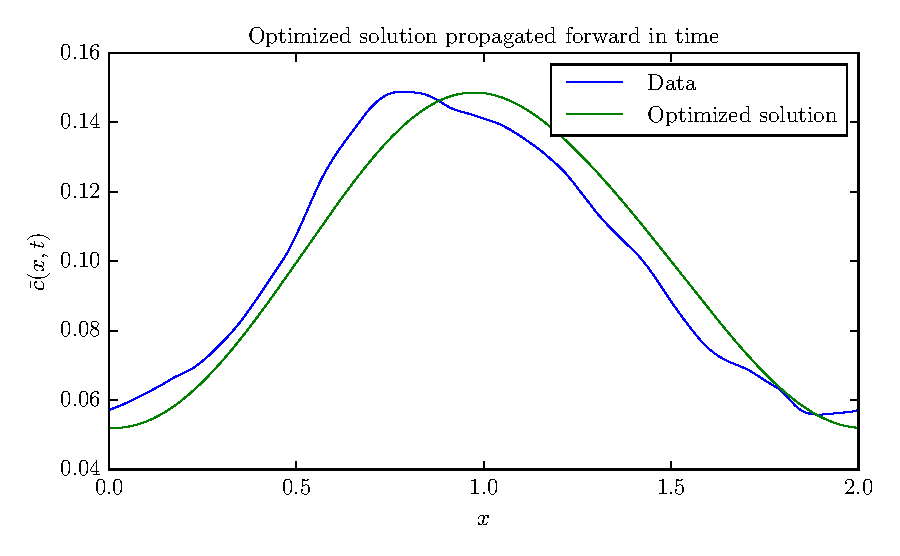
\includegraphics[width=0.4\textwidth]{figs/solnPropagated_t1.pdf}
  \end{figure}
  Prediction could be better.  This motivates use of a stochastic forward
  operator.
\end{frame}

\end{document}
